\minitoc

\vfill

As seen in the previous chapter, some error labels are poorly detected with the baseline features.
The aim here is to present a new set of features so as to achieve better prediction scores.
First, Section~\ref{sec::better_representation::literature}, we introduce some advanced feature extractors from the literature that can fit our experimental constraints.
In Section~\ref{sec::better_representation::evaluation}, we show how these ideas are utilized in our evaluation workflow.
Last, Section~\ref{sec::better_representation::implementation} presents the implementation details related to these advanced feature extractors.

\clearpage

\section{Image and graph classification in the literature}
    \label{sec::better_representation::literature}
    In this section, we review two state-of-the-art tools that are used to extract better features of \gls{acr::3d} models.
    First, we present the \gls{acr::scatnet} which can be seen as a \gls{acr::cnn} emulator.
    Second, we show how kernels could be used to classify graphs in the literature.

    \subsection{\acrshort*{acr::scatnet} for image classification}
        \label{subsec::better_representation::literature::scatnet}
        \acrfullpl{acr::scatnet} can be seen as a reverse engineered convolutional network.
        They are built mainly relying on wavelet filters which are used to imitate filters from \glspl{acr::cnn}.
        The latter learns automatically an image representation $\Phi$ trying to minimize a learning loss function.
        \Glspl{acr::scatnet}, on the other hand, make use of mathematical properties of the image signal.\\

        Some properties are always required in order to achieve a good representation $\Phi$ of an image. 
        A scene that is captured from different points of view, while yielding different images, should have close representations.
        Just as with intersect point detection~\parencite{lowe2004distinctive}, the representation of an image should be invariant to scale, translation and rotation~\parencite{mallat2012group,sifre2013rotation,bruna2013invariant}.
        Since images illustrate not only rigid objects, a good representation should allow small local deformations in the signal that can be attributed to distortions of non-rigid objects.\\

        \subsubsection{Mathematical notations.}
            To formalize these properties, we introduce some mathematical notations.
            \paragraph{Action of a group.}
                Let $x: u \mapsto x(u)$ be an image (or any signal in general) and $(G, *)$ a group such as, for example, the set of translation operators on signals.
                The action of $g\in G$ on $x$ is written as:
                \begin{equation}
                    \label{eq::action_group}
                    L_g(x): u \mapsto x\left(g^{-1}(u)\right).
                \end{equation}
            
                As an example, we can study the case of $T_{\mathbb{R}^2}$ a translation group on $\mathbb{R}^2$.
                This group is isomorphic to $\mathbb{R}^2$: i.e., $(T_{\mathbb{R}^2}, \circ) \cong (\mathbb{R}^2, +)$.
                Let $v$ be a vector in $\mathbb{R}^2$.
                We denote a translation by vector $v$ by $t_v: u \mapsto u + v$.
                Its inverse verifies $t_v^{-1} = t_{-v}$.
                For $v \in \mathbb{R}^2$, we can express the translation applied to signal as:
                \begin{equation}
                    \label{eq::action_translation}
                    L_{t_v}(x): u \mapsto x\left(u - v\right).
                \end{equation}
                Equally, if we consider the rotation group $SO(2)$ which is isomorphic to the unit circle, and write a rotation of angle $\theta \in [0, 2\cdot\pi)$ as $r_{\theta}$, we express the action of that group as:
                \begin{equation}
                    \label{eq::action_rotation}
                    L_{r_{\theta}}(x): u \mapsto x\left(r_{-\theta}(u)\right).
                \end{equation}
                Rotations and translations are not commutative in the general case.
                This justifies the definition of a roto-translation group, called also the rigid motion group and denoted $SE(2)$.
                Such a group is isomorphic to $\mathbb{R}^2 \times SO(2)$.
                Let $v \in \mathbb{R}^2$ and $\theta \in [0, 2\cdot\pi)$, a member of such a group is defined as:
                \begin{equation}
                    \label{eq::roto-translation}
                    g_{\theta, v} \triangleq t_v \circ r_{\theta} = r_{\theta} \circ t_{r_{-\theta}(v)}
                \end{equation}
                and its inverse is expressed then as $g_{\theta, v}^{-1} = r_{-\theta} \circ t_{-v}$.
                Hence we can write:
                \begin{equation}
                    \label{eq::action_roto-translation}
                    L_{g_{\theta, v}}(x): u \mapsto x \left(r_{-\theta}(u - v)\right).
                \end{equation}
            
            \paragraph{Group convolution.}
                A convolution over a locally compact topological group $G$ is defined as:
                \begin{equation}
                    \label{eq::group_signal_convolution}
                    x \ostar y: u \mapsto \int_{h\in G} x(h)\cdot y(h^{-1}(u)) \cdot dh
                \end{equation}
                where:
                \begin{conditions}
                    dh & is the Haar measure on $G$.
                \end{conditions}

                For signals $x$ and $y$ that take inputs on the plane $\mathbb{R}^2$, we can recognize the usual definition of a convolution:
                \begin{equation}
                    \label{eq::translation_convolution}
                    x \star y: u \mapsto \int_{v \in \mathbb{R}^2} x(v)\cdot y(u - v) \cdot dv
                \end{equation}

                Applied in the roto-translation case to signals $x(u, \theta)$ on pairs from $\mathbb{R}^2 \times [0, 2\cdot\pi)$, we write:
                \begin{equation}
                    \label{eq::roto-translation_convolution}
                    x \ostar_{SE(2)} y: (u, \theta) \mapsto \int_{\substack{v \in \mathbb{R}^2\\\omega \in [0, 2\cdot\pi)}} x(v, \omega)\cdot y(r_{-\omega}(u - v), \theta - \omega) \cdot dv d\omega
                \end{equation}

        \subsubsection{Invariance: formulation.}
            $\Phi$ is said to be invariant to $g$ if and only if:
            \begin{equation}
                \label{eq::invariance}
                \Phi\circ L_g\left(x\right) = \Phi(x),
            \end{equation}
            and covariant if and only if:
            \begin{equation}
                \label{eq::covariance}
                \Phi\circ L_g\left(x\right) = L_g\circ\Phi(x).
            \end{equation}
            Images of similar objects should have also similar representations.
            Using Euclidean distances as a similarity measure, this property implies $\Phi$ to be contractive~\parencite{bruna2013invariant}.
            Given two images $x$ and $y$, we write:
            \begin{equation}
                \label{eq::contractive}
                \Vert \Phi(x) - \Phi(y) \Vert \leq \Vert x-y \Vert.
            \end{equation}
            The mapping $\Phi$ should be stable under small local deformations.
            A local deformation is modeled as a diffeomorphism\footnote{A differentiable bijection which inverse is also differentiable.} $\tau$.
            A small one is formalized as a diffeomorphism $\tau$ that verifies $\Vert\nabla \tau\Vert_\infty < 1$~\parencite{mallat2012group,bruna2013invariant,sifre2013rotation}.
            Consequently a good transform $\Phi$ should be Lipschitz stable to deformations:
            \begin{equation}
                \label{eq::stable_deformation}
                \exists C >0, \forall x \in \mathscr{I}\quad \Vert \Phi(x) - \Phi\circ L_\tau(x) \Vert \leq C \cdot \Vert x\Vert \cdot \Vert\nabla \tau\Vert_\infty.
            \end{equation}
            where:
            \begin{conditions}
                \mathscr{I} & is the set of all possible signals;\\
                L_\tau(x) & $u \mapsto x(u - \tau(u))$ is the action of the deformation $\tau$ on a signal $x$.
            \end{conditions}

        \subsubsection{\gls*{acr::scatnet}: a reverse engineered \gls*{acr::cnn}.}
            \glspl{acr::cnn} learn such a representation in the hopes of verifying these previous conditions stated in Equations~\ref{eq::contractive},~\ref{eq::invariance} and~\ref{eq::stable_deformation}.
            In fact, it is possible by virtue of some basic building blocs.
            First, since the weights are learned based on a classification objective, images with similar content are supposed to be mapped to the same region.
            Secondly, pooling layers in \glspl{acr::cnn} provide a solution for invariance to translations and local deformations up to a scale.\\

            \glspl{acr::scatnet} formalize these ideas using wavelet transforms.
            Actually, \glspl{acr::scatnet} were originally developed to better understand \glspl{acr::cnn}.
            The idea is to apply linear convolutional operators followed by a non-linearity and some pooling operators.
            In a \gls{acr::scatnet} the learned filters are replaced by a specific wavelet decomposition, the non-linearity is achieved using the modulus operator and pooling is obtained through a low pass filter.
            The low-pass filter is critical for the invariance condition, while the lost high frequencies are retrieved using the wavelet convolutions.
            The non-linearity, just as in \glspl{acr::cnn}, is necessary in order to obtain interesting non-linear final representations.\\

            \paragraph{Wavelets filter bank.}
                We need two sets of wavelets: spatial and angular ones.
                Spatial wavelet filters are derived based on a mother wavelet $\psi: \mathbb{R}^2 \rightarrow \mathbb{C}$ as follows:
                \begin{equation}
                    \label{eq::translation_filter_bank}
                    \psi_{i,\theta} : u\mapsto 2^{-2\cdot i}\cdot\psi\left(2^{-i}\cdot r_{-\theta}(u)\right).
                \end{equation}
                We also need a low-pass averaging filter $\phi: \mathbb{R}^2 \rightarrow \mathbb{R}$ scaled up to a desired size:
                \begin{equation}
                    \label{eq::translation_low_pass}
                    \phi_I: u\mapsto 2^{-2\cdot I}\cdot\phi\left(2^{-I}\cdot u\right)
                \end{equation}
                The angular wavelets are computed using $2\cdot\pi$-periodic mother wavelet $\bar\psi: \mathbb{R}^2 \rightarrow \mathbb{C}$ scaled as follows:
                \begin{equation}
                    \label{eq::angular_filter_bank}
                    \bar\psi_{\xi}: \omega \mapsto 2^{-\xi}\cdot\bar\psi\left(2^{-\xi}\cdot \omega\right)
                \end{equation}
                We also define the constant averaging filter\footnote{It corresponds to a zero scale filter.} defined as:
                \begin{equation}
                    \label{eq::angular_low_pass}
                    \bar\phi: \theta \mapsto \frac{1}{2\cdot\pi}
                \end{equation}
                Based on the spatial filter bank defined in Equation~\ref{eq::translation_filter_bank} and the angular one from Equation~\ref{eq::angular_filter_bank}, we define rigid motion wavelets in the next equations:
                \begin{align}
                    \label{eq::roto-translation_filter_bank}
                    \forall i\neq I, \theta \neq 0, \xi \neq 0 \quad \tilde{\psi}_{i, \theta, \xi}(u, \omega) &= \psi_{i,\theta}(u) \cdot \bar\psi_{\xi}(\omega)\\
                    \forall \xi \neq 0 \quad \tilde{\psi}_{I, 0, \xi}(u, \omega) &= \phi_I(u) \cdot \bar\psi_{\xi}(\omega)\\
                    \forall i\neq I, \theta \neq 0 \quad \tilde{\psi}_{i, \theta, 0}(u, \omega) &= \psi_{i,\theta}(u) \cdot \bar\phi(\omega).
                \end{align}
                The corresponding rigid motion averaging filter is obtained as:
                \begin{align}
                    \label{eq::roto-translation_low_pass}
                    \tilde{\phi}(u, \omega) &= \tilde{\psi}_{I, 0, 0}(u, \omega) = \phi_I(u) \cdot \bar\phi(\omega) \nonumber \\
                    \tilde{\phi}(u, \omega) &= \frac{1}{2\cdot\pi} \cdot \phi_I(u)
                \end{align}
                These are separable filters that can help speed up the convolution computations as shown in~\textcite{sifre2013rotation}.
                In practice, $\psi$(\textit{resp.} $\bar\psi$) are taken as two (\textit{resp.} one) dimensional Morlet wavelets (cf. Figure~\ref{subfig::morlet_filters}), while $\phi$ is taken as a Gaussian~\parencite{sifre2013rotation,bruna2013invariant,oyallon2015deep}.
                A finite number $L$ of orientations are possible for angle indices: $\theta \in \left\{\frac{l\cdot\pi}{L}: l=1,2\dots,L\right\}$.
                In Figure~\ref{fig::morlet_vs_learned}, we can see how the designed filter bank is similar to the one learned by a \gls{acr::cnn}.
                \begin{figure}
                    \centering
                    \ffigbox{
                        \ffigbox[\FBwidth]{
                            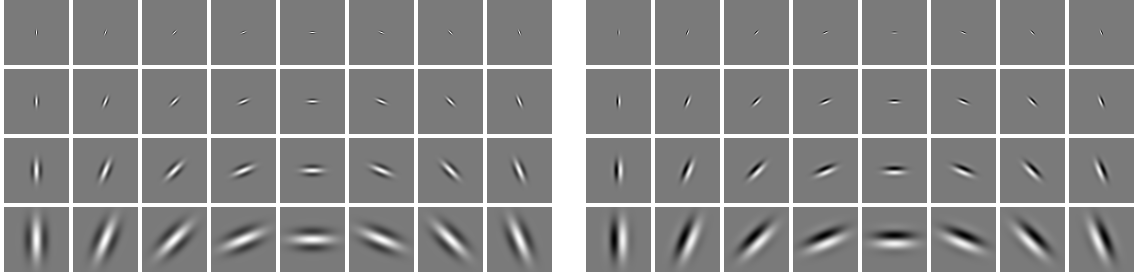
\includegraphics[width=\textwidth]{images/related_work/morlet_wavelets}
                        }{
                            \caption[
                                Morlet wavelets at different scales ($I=5$) and orientations ($L=8$).
                            ]{
                                \label{subfig::morlet_filters}
                                Morlet wavelets at different scales ($I=5$) and orientations ($L=8$).
                                Left are presented the real parts while the imaginary parts are on the right.
                                Image taken from~\parencite{sifre2013rotation}.
                            }
                        }
                        \ffigbox[\FBwidth]{
                            \begin{tabular}{@{}c@{}}
                                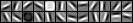
\includegraphics[width=.5\textwidth]{images/related_work/first_layer_cnn}\\
                                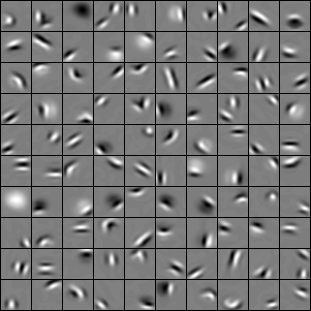
\includegraphics[width=.75\textwidth]{images/related_work/second_layer_cnn}
                            \end{tabular}
                        }{
                            \caption[
                                Learned filters at the first and second layers of a \acrshort*{acr::cnn}.
                            ]{
                                \label{subfig::learned_filters}
                                Learned filters at the first (top) and second (bottom) layers of a \gls{acr::cnn}.
                                Image taken from~\parencite{lee2009convolutional}.
                            }
                        }
                    }{
                        \caption[
                            Comparison of the Morlet wavelet bank and the first and second layer filters learned from a \acrshort*{acr::cnn}.
                        ]{
                            \label{fig::morlet_vs_learned}
                            Comparison of the Morlet wavelet bank and the first and second layer filters learned from a \gls{acr::cnn}.
                            The latter can be distinguished into two classes:
                            an averaging filter that could be likened to $\phi$ and rotated and scaled (only in the second layer) filters that looks like Morlet wavelets.
                        }
                    }
                \end{figure}
                
            \paragraph{The wavelet-modulus operator.}
                A wavelet transform of a signal $x$ consists in representing it using a wavelet filter bank: $\left(x\ostar\psi_{\lambda}\right)_{\lambda}$.
                Depending on the transformed signals, two versions of wavelet transforms are possible.
                If the signal takes one variable $u \in \mathbb{R}^2$ then we write:
                \begin{equation}
                    \label{eq::wavelet_transform_1}
                    W: x \mapsto \left(x\star\psi_{i, \theta}\right)_{\substack{i=1, 2 \dots, I \\ \theta \in \left\{\frac{l\cdot\pi}{L}: l=1,2\dots,L\right\}}},
                \end{equation}
                if it takes two variables $(u, \omega) \in \mathbb{R}^2 \times [0, 2\cdot\pi)$ it becomes:
                \begin{equation}
                    \label{eq::wavelet_transform_2}
                    \widetilde{W}: x \mapsto \left(x\ostar_{SE(2)}\psi_{i, \theta, \xi}\right)_{\substack{i=1, 2 \dots, I \\ \theta \in \left\{\frac{l\cdot\pi}{L}: l=1,2\dots,L\right\}\\\xi=1,2\dots,\lfloor\log_2(L)\rfloor}}.
                \end{equation}
                An image is a discretization of a two dimensional signal.
                As a consequence, we can only apply the first transform in Equation~\ref{eq::wavelet_transform_1}.
                The result of such a mapping is an example of a signal to which one can apply the second transform from Equation~\ref{eq::wavelet_transform_2}.
                For the right choice of wavelets, these operators can be proven to be invertible, contractive and Lipschitz stable to deformations~\parencite{mallat2012group}.\\

                By applying a modulus we get the basic building bloc of \glspl{acr::scatnet} called the wavelet-modulus operator: $x \mapsto \vert x\ostar\psi_{\lambda} \vert$.
                This is delineated for the two cases as follows:
                \begin{align}
                    \label{eq::wavelet-modulus_1_2}
                    U_{i, \theta}: x &\mapsto \vert x\star\psi_{i, \theta}\vert\\
                    \widetilde{U}_{i, \theta, \xi}: x &\mapsto \vert x\ostar_{SE(2)}\psi_{i, \theta, \xi} \vert
                \end{align}
                These operators are proven to be covariant to translations and rotations~\parencite{mallat2012group,sifre2013rotation}: i.e., for a couple $(v, \vartheta) \in \mathbb{R}^2 \times [0, 2\cdot\pi)$:
                \begin{align}
                    \label{eq::covariance_wavelet-modulus}
                    L_{g_{v, \vartheta}} \circ U_{i, \theta} &= U_{i, \theta} \circ L_{g_{v, \vartheta}}\\
                    L_{g_{v, \vartheta}} \circ \widetilde{U}_{i, \theta, \xi} &= U_{i, \theta, \xi} \circ L_{g_{v, \vartheta}}.
                \end{align}
                These conditions may remind the reader of the work of~\textcite{cohen2016group} on \gls{acr::gcnn}.
            
            \paragraph{The average pooling.}
                Contrarily to~\parencite{cohen2016group}, the pooling operations differ.
                \glspl{acr::gcnn} rely on max-pooling as standard practice in \glspl{acr::cnn}.
                This operator is actually covariant to actions of the rigid movement group.
                \parencite{bruna2013invariant, sifre2013rotation,oyallon2015deep}, however, rely on averaging (or low-pass) filters as pooling operators.

                Considering the rigid movement as a nuisance,~\parencite{sifre2013rotation} considers invariance with regards to the roto-translation group.
                To do so they filter any signal $x(u)$ using $\phi_I$ yielding a signal:
                \begin{equation}
                    \label{eq::pool_bi-dim}
                    P_I: x \mapsto x \star \phi_I (u).
                \end{equation}
                For signals $\tilde{x}(u, \omega)$ they are averaged using $\tilde{\phi}_I$ and giving as ouput:
                \begin{equation}
                    \label{eq::pool_bi-dim-angular}
                    \widetilde{P}_I: x \mapsto \tilde{x} \ostar_{SE(2)} \tilde{\phi}_I (u, \omega).
                \end{equation}

                These operators are actually invariant to translation and rotation:
                \begin{align}
                    \label{eq::invariance_pooling}
                    P_I = P_I \circ L_{t_v}\\
                    \tilde{P}_I = \tilde{P}_I \circ L_{g_{v, \vartheta}}.
                \end{align}

            \paragraph{Scattering coefficients.}
                Applying the first operation~\ref{eq::pool_bi-dim} to the input image defines the first scattering coefficient:
                \begin{equation}
                    \label{eq::scatter_input}
                    S_0[x](u) \triangleq x \star \phi_I (u).
                \end{equation}
                
                To the image, the wavelet-modulus operator is applied giving coefficients $U_{i_1, \theta_1}(x)$.
                The latter is averaged using the second operation from Equation~\ref{eq::pool_bi-dim-angular}.
                This defines the second layer of scattering coefficients:
                \begin{equation}
                    \label{eq::scatter_first}
                    S_1[x](u, i_1, \theta_1) \triangleq U_{i_1, \bullet} \ostar_{SE(2)} \tilde{\phi}_I(u, \theta_1).
                \end{equation}

                At the second level is applied the wavelet-modulus operator retrieving the high-frequencies lost after the low-pass filter using yet another time the wavelet-modulus operator yielding:
                \begin{equation}
                    \label{eq::cascade_second}
                    \widetilde{U}_{i_2,\xi_2, \theta_2} \circ U_{i_1, \theta_1}(x)
                \end{equation}
                Once again, an average pooling is applied to the latter:
                \begin{equation}
                    \label{eq::scatter_second}
                    S_2[x](u, i_1, \theta_1, i_2, \theta_2, \xi_2) \triangleq \widetilde{U}_{i_2,\xi_2, \theta_2} \circ U_{i_1, \bullet} \ostar_{SE(2)} \tilde{\phi}_I(u, \theta_1).
                \end{equation}
                
                This can be reapplied further giving cascaded scattering coefficients at level $m$:
                \begin{equation}
                    \label{eq::scatter_second}
                    S_m[x](u, p_m) \triangleq \widetilde{U}_{\lambda_m} \circ \widetilde{U}_{\lambda_{m-1}} \dots \circ \widetilde{U}_{\lambda_2} \circ U_{i_1, \bullet} \ostar_{SE(2)} \tilde{\phi}_I(u, \theta_1).
                \end{equation}
                where:
                \begin{conditions}
                    p_m & $i_1, \theta_1, \lambda_2 \dots, \lambda_{m-1}, \lambda_m$ and is called a path;\\
                    \lambda_k & $i_k, \theta_k, \xi_k$.
                \end{conditions}

                The scattering coefficients are proved to be contractive and Lipschitz stable to deformations~\parencite{mallat2012group}.
                Moreover, they are invariant to actions of the group of rigid movement.
                In fact, concatenating a covariant operator and an invariant one yields an invariant operator~\parencite{mallat2012group,sifre2013rotation}.

                The energy of the signal is concentrated along increasing scale paths: i.e., $\forall k = 1, 2, \dots, m-1 \; i_{k+1} > i_k$.
                This implies that computing coefficients along these paths is sufficient~\parencite{bruna2013invariant,sifre2013rotation,oyallon2015deep}.
                Furthermore, only the first two layers are computed as they concentrate most the energy of the signal~\parencite{bruna2013invariant,sifre2013rotation,oyallon2015deep}.
                This yields an efficient way of computing a scattering transform as discussed by~\textcite{sifre2013rotation,oyallon2015deep}.
                This means that total number of the possible paths is in practice:
                \begin{equation}
                    \label{eq::scatnet_number_paths}
                    n_S = \underbrace{1}_{\substack{\text{layer}\\l = 0}} + \underbrace{L \cdot I}_{\substack{\text{layer}\\l = 1}} + \underbrace{\frac{L^2\cdot I \cdot \left(I - 1\right)}{2}}_{\substack{\text{layer}\\l = 2}}.
                \end{equation}

                \textcite{sifre2013rotation} go on to propose a way to make the scattering invariant to scale effects also.
                This is done by introducing a logarithm that linearizes the dependency of scattering coefficients to scales $i_1$ and $i_2$~\parencite{sifre2013rotation,oyallon2015deep}.
                A scale-space averaging is thus applied to achieve the sought invariance~\parencite{sifre2013rotation}.\\

                In contrast,~\textcite{oyallon2015deep} propose to keep only the translation invariance and let the classifier decide on the relevance of rotation and scale invariance, much like in~\parencite{cohen2016group}.
                To do so only a spatial averaging convolution is applied as $x \mapsto \tilde{x}(\bullet, \omega) \star \phi_I$ which is covariant to rotations.
                Similarly, they drop the scale-space averaging at the end, while the logarithm guaranties the covariance of the signal to scaling effects.
                The operations are also conducted in a way that renders the shape of the \gls{acr::scatnet}, shown in Figure~\ref{fig::scatnet}, more like that of \gls{acr::cnn}.

                \begin{figure}[htbp]
                    \centering
                    \includestandalone[mode=buildnew, width=\textwidth]{figures/scattering_network}
                    \caption[
                        Illustration of a \acrshort*{acr::scatnet}.
                    ]{
                        \label{fig::scatnet} Illustration of a \gls{acr::scatnet}.
                        At each level are computed convolutions with a filter bank followed by a modulus operator.
                        The scattering coefficients are obtained then by a low-pass filter (in blue).
                        In practice, scattering coefficients are only computed for increasing scale paths up to level $2$.
                    }
                \end{figure}

    \subsection{Kernels for graph classification}
        \label{subsec::better_representation::literature::graph_classification}
        Standard machine learning practice usually assumes that the observed instances live in a finite dimensional space.
        This is not always the case.
        In fact, graphs can have varying numbers of nodes and edges.
        Moreover, they can be different while providing the same structural information: we say they are isomorphic.
        A valid representation for graphs should then take care of these two issues: incorporate all possible graph sizes and be invariant to graph isomorphisms.
        As accustomed in statistical learning, one way to alleviate these issues is to directly compare graphs using kernels as seen previously in Section~\ref{subsubsec::state_of_the_art::mlpr::classifiers::svm}.\\

        This Section does not aim at presenting a thorough survey of graph kernels.
        The work of~\textcite{ghosh2018journey} categorizes graph kernels depending on the used methodology.
        A different approach is proposed in~\textcite{kriege2020survey}, where graph kernels are studied based on the underlying graphs.\\

        Apart from the structure of the graph, kernels should also take into account the labels or continuous attributes assigned to a graph.
        These could be given at node level or edge level.
        We will present hereafter some graph kernels which were used in this work, namely, continuously node attributed ones, as well as those devoted only to its structural properties.\\

        \subsubsection{Basic kernels.}
            Let $G = \left(V, E\right)$ be an undirected graph with vertices $v\in V$ and edges $e \in E =\left\{\left\{u, v\right\}: (u, v) \in V\times V\right\}$.
            Attributes can be associated to each node $a: V \rightarrow \mathbb{R}^{d_V}$ or edge $b: E \rightarrow \mathbb{R}^{d_E}$.\\

            The most basic graph kernel would correspond to a scalar product of a global hashing vector of all attributes.
            This is possible through the use of a histogram function for instance.
            This type of functions is described in details in Section~\ref{subsec::learned_evaluation::baseline::geometric}.\\

            Let $S\left(\left(a(v)_i\right)_{v\in V}\right): \mathbb{R}^{\vert V\vert} \rightarrow \mathbb{R}^l$ (\textit{resp.} $S\left(\left(b(e)_i\right)_{e\in E}\right): \mathbb{R}^{\vert E\vert} \rightarrow \mathbb{R}^{m}$) be a hashing function that describes the distribution of attributes $i$ of all nodes (\textit{resp.} edges) of graph $G$ as a $\mathbb{R}^{l_i}$ (\textit{resp.} $\mathbb{R}^{m_i}$) vector.
            We can build a node based feature vector for the graph $G$:
            \begin{equation}
                \label{eq::feature_node_graph}
                \Phi_V(G) \triangleq \begin{bmatrix}
                    S\left(\left(a(v)_1\right)_{v\in V}\right)\\
                    S\left(\left(a(v)_2\right)_{v\in V}\right)\\
                    \vdots\\
                    S\left(\left(a(v)_{d_V}\right)_{v\in V}\right)
                \end{bmatrix} \in \mathbb{R}^{d_V \cdot l}
            \end{equation}
            and an edge based one:
            \begin{equation}
                \label{eq::feature_edge_graph}
                \Phi_E(G) \triangleq \begin{bmatrix}
                    S\left(\left(b(e)_1\right)_{e \in E}\right)\\
                    S\left(\left(b(e)_2\right)_{e \in E}\right)\\
                    \vdots\\
                    S\left(\left(b(e)_{d_E}\right)_{e \in E}\right)
                \end{bmatrix} \in \mathbb{R}^{d_E \cdot m}.
            \end{equation}

            Based on a base kernel on vectors $\kappa$ (cf. Section~\ref{subsubsec::state_of_the_art::mlpr::classifiers::svm}), we can compute the similarity between two graphs $G = \left(V, E\right)$ and $G' = \left(V', E'\right)$:
            \begin{align}
                \label{eq::feature_graph_kernel_nodes}
                k_V(G, G') &\triangleq \kappa(\Phi_V(G), \Phi_V(G'))\\
                \label{eq::feature_graph_kernel_edges}
                k_E(G, G') &\triangleq \kappa(\Phi_E(G), \Phi_E(G')).
            \end{align}
            Concatenating both feature vectors would amount to a simple addition of these kernels:
            \begin{equation}
                \label{eq::feature_graph_kernel_sum}
                k(G, G') \triangleq k_V(G, G') + k_E(G, G').
            \end{equation}

            This type of kernels is versatile as it can be applied to node and edge attributes as well as labels (with the right choice of hashing function).
            However, it does not take into account the structure of the graph.
            It is mainly used as a baseline for graph feature extraction.
            The work of~\textcite{shervashidze2011weisfeiler} is an example of kernels that uses the same idea to describe graphs while taking account of their structure.

        \subsubsection{Random walk kernel.}
            In order to define this kernel, we need to define the adjacency matrix $A$ of a graph $G$:
            \begin{equation}
                \label{eq::adjacency_matrix}
                A \triangleq \left(\delta_{\left\{u,v\right\}\in E}\right)_{(u, v) \in V\times V}
            \end{equation}
            and the diagonal matrix of node degrees $D\triangleq \operatorname{diag}\left(\sum_{v \in V}A_{uv}\right)_{u \in V}$.
            We also denote the normalized adjacency matrix as:
            \begin{equation}
                \label{eq::normalized_adjacency_matrix}
                P \triangleq A\cdot D^{-1}
            \end{equation}

            The latter could be interpreted as a transition probability matrix of a random walk on the graph:
            $P_{uv}$ is the probability of choosing $u$ as the next node to visit starting from $v$.
            Similarly, $\left(P^k\right)_{uv}$ expresses the probability of being in node $u$ after $k$ iterations, starting from $v$.
            A random walk starts with an initial distribution $p$ over the nodes.
            After $k$ iterations, the distribution is $P^k\cdot p$.
            At any time, the walk can end with a probability $q_u$ at node $u$.
            $p$ and $q$ are used to encode prior information of the graph~\parencite{vishwanathan2010graph}.\\
            
            \paragraph{Simultaneous random walk.}
                To compare two graphs \(G\) and \(G'\) using random walks, we start by defining the direct product graph $G_{\times} = \left(V_{\times}, E_{\times}\right)$ where:
                \begin{align}
                    \label{eq::direct_product_graph}
                    V_{\times} &\triangleq V \times V'\\
                    E_{\times} &\triangleq \left\{\left\{(u, u'), (v, v')\right\}: \left\{u,v\right\} \in E \wedge \left\{u',v'\right\} \in E'\right\}.
                \end{align}
                This is vizualized in Figure~\ref{fig::direct_product_graph}.
                \begin{figure}[htbp]
                    \centering
                    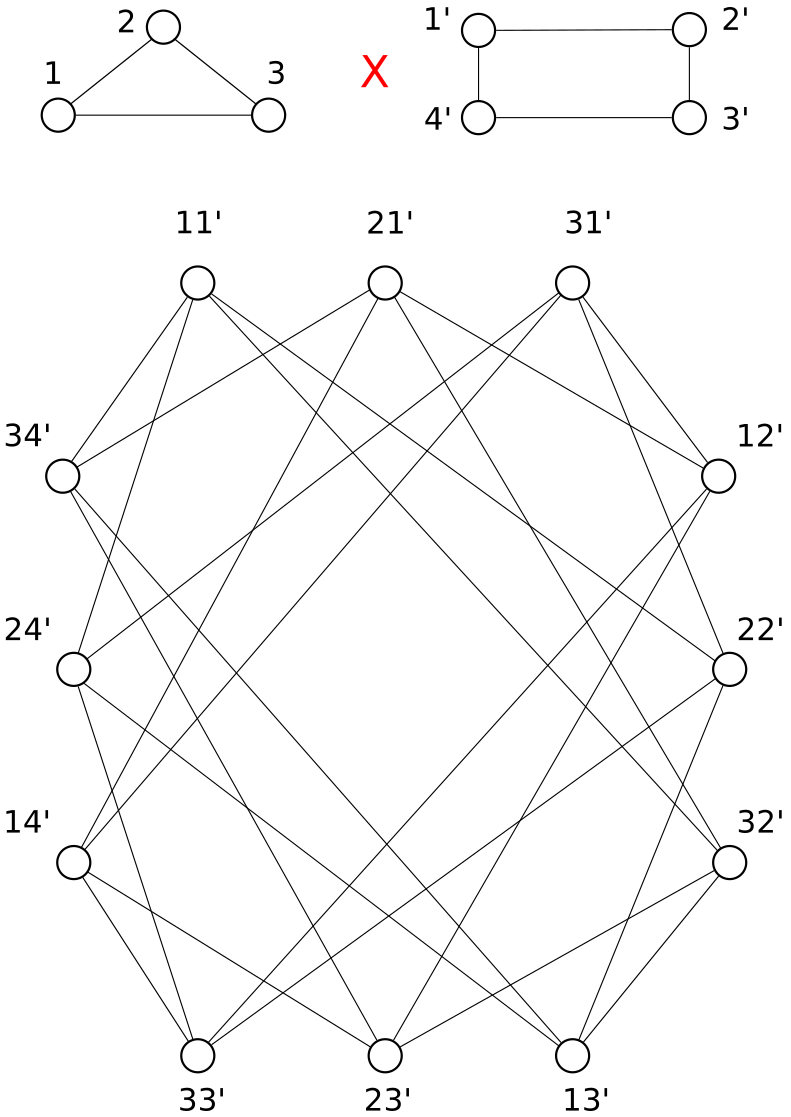
\includegraphics[height=.4\textheight]{images/related_work/direct_product_graphs}
                    \caption[
                        Depiction of a direct product of two graphs.
                    ]{
                        \label{fig::direct_product_graph}
                        Depiction of a direct product (bottom) of two graphs (top).
                        Nodes adjacent in the direct product graph $G_{\times}$ correspond to adjacent nodes in both graphs.
                        Image taken from~\parencite{vishwanathan2010graph}.
                    }
                \end{figure}

                For the direct product graph, we compute adjacency matrices, initial probability distribution and stopping probabilities as follows:
                \begin{align}
                    \label{eq::direct_product_graph_walk}
                    A_{\times} &= A \otimes A'\\
                    P_{\times} &= P \otimes P'\\
                    p_{\times} &= p \otimes p'\\
                    q_{\times} &= q \otimes q'
                \end{align}
                where:
                \begin{conditions}
                    \otimes & refers to the Kronecker product.
                \end{conditions}
                In fact, a random walk on $G_{\times}$ is equivalent to a simultaneous random walk on $G$ and $G'$~\parencite{hammack2011handbook}.\\

                A random walk on a graph depends heavily on the its structure.
                In consequence, a random walk on the direct product graph can be used as an indicator of the similarity in structure of both graphs $G$ and $G'$.
                It is defined as:
                \begin{equation}
                    \label{eq::random_walk_kernel}
                    k_{rw}(G, G') \triangleq \sum_{k=0}^\infty \lambda_k \cdot q_{\times}^\intercal\cdot P_{\times}\cdot p_{\times}.
                \end{equation}
                The choice of the series $\left(\lambda_k\right)_{k\in \mathbb{N}}$ is critical, as the kernel defined in Equation~\ref{eq::random_walk_kernel} can diverge.
                It is taken to be non-negative in order in ensure the positive semi-definite of the kernel.\\

            \paragraph{Special cases.}
                This defintion actually generalizes a family of graph kernels based on walks on graphs~\parencite{vishwanathan2010graph}.
                Setting $p_{\times} \propto 1$ and $q_{\times} \propto 1$ and, there are two cases of interest:
                \begin{itemize}
                    \item Let \(\lambda \in \mathbb{R}^*_+\), we set \(\forall k\in \mathbb{N} \; \lambda_k = \lambda^k\): this gives rise to a geometric random kernel:
                            \begin{equation}
                                \label{eq::geometric_random_kernel}
                                k_{grw}(G, G') = \begin{bmatrix}
                                    1, 1\dots,1
                                \end{bmatrix}\cdot \left(I - \lambda\cdot A_{\times}\right)^{-1}\cdot\begin{bmatrix}
                                    1\\
                                    1\\
                                    \vdots\\
                                    1
                                \end{bmatrix}.
                            \end{equation}
                            Let \(\lambda_{\times}\) the largest eigenvalue of \(A_{\times}\).
                            For this kernel to be valid, the following condition must hold:
                            \begin{equation}
                                \label{eq::condition_geometric_kernel_convergence}
                                \lambda < \frac{1}{\lambda_{\times}}
                            \end{equation}
                    \item Let \(\lambda \in \mathbb{R}^*_+\), we set \(\forall k\in \mathbb{N} \; \lambda_k = \frac{\lambda^k}{k!}\): this yields the so called exponential random kernel:
                            \begin{equation}
                                \label{eq::geometric_random_kernel}
                                k_{erw}(G, G') = \begin{bmatrix}
                                    1, 1\dots,1
                                \end{bmatrix}\cdot \exp\left(\lambda\cdot A_{\times}\right)\cdot\begin{bmatrix}
                                    1\\
                                    1\\
                                    \vdots\\
                                    1
                                \end{bmatrix}.
                            \end{equation}
                \end{itemize}
                These graph kernels were already defined in~\parencite{gartner2003graph}.\\

            Computationally, these kernels involve heavy computations.
            \textcite{vishwanathan2010graph} proposed efficient numerical algorithms to alleviate this problem.
            However, these graphs suffer from other issues.
            First, the kernel does take into account the attributes of graphs if they exist, although it is possible to adapt.
            Secondly, these kernels suffer from tottering.
            The latter being the fact that random walks are mostly consistent of multiple movements between a small subset of vertices in a row.
            Third, related to the previous point, the random walk would spend much time on central nodes that connect to most other nodes adding to their contribution to the kernel, while peripherial ones that can hold the most distinctive feature of the structure are watered down.
            It is possible to address these issues as demonstrated by~\textcite{horvath2004cyclic, mahe2004extensions}.
            However these kernels cannot be guaranteed to be computed in polynomial time~\parencite{vishwanathan2010graph}.

        \subsubsection{\gls*{acr::svm} $\vartheta$ kernel.}
            This is also a kernel which takes advantage only of the structure of graphs.
            It relies on the definition of Lov\'asz number of a graph $\vartheta(G)$.
            For each vertex $v \in V$, we can assign a unit vector \(\bm{w}_v \in \left\{u \in \mathbb{R}^d: \left\lVert u \right\rVert = 1 \right\}\).
            The set of vectors \(W(G) \triangleq \left(\bm{w}_v\right)_{v \in V}\) is said to be an orthonormal representation of a graph $G$ if and only if:
            \begin{equation*}
                \forall \left\{u,v\right\} \notin E \Rightarrow \bm{w}_u^\intercal\cdot \bm{w}_v=0.
            \end{equation*}

            \paragraph{Lov\'asz $\vartheta$ kernel.}
                The Lov\'asz number~\parencite{lovasz1979shannon} is defined as:
                \begin{equation}
                    \label{eq::lovazs_number}
                    \vartheta(G) \triangleq \min_{\substack{\bm{c} \in \mathbb{R}^d\\W(G)}}\max_{v\in V} \left(\frac{1}{\bm{c}^\intercal\cdot \bm{w}_v}\right)^2
                \end{equation}
                Which can be interpreted as the smallest cone enclosing a valid orthonormal representation of graph $G$.\\
                Equally, we define the Lov\'asz number over a subset of vertices $B \in V$ as follows:
                \begin{equation}
                    \label{eq::lovazs_number_subset}
                    \vartheta_B(G) \triangleq \min_{\bm{c} \in \mathbb{R}^d}\max_{\bm{w}_v\in W_B^*(G)} \left(\frac{1}{\bm{c}^\intercal\cdot \bm{w}_v}\right)^2
                \end{equation}
                where:
                \begin{conditions}
                    W^*_B(G) & is the restriction of $W^*(G)$ over the subset $B$;\\
                    W^*(G) & is the maximizer of the problem in Equation~\ref{eq::lovazs_number}.
                \end{conditions}

                The Lov\'asz kernel~\parencite{johansson2014global} is defined based on a base kernel $\kappa: \mathbb{R} \times \mathbb{R} \rightarrow \mathbb{R}_+$ as:
                \begin{equation}
                    \label{eq::lovazs_number_kernel}
                    k_{\vartheta}(G, G') \triangleq \sum_{\substack{B\subseteq V\\B'\subseteq V'\\\vert B \vert = \vert B' \vert}} \frac{1}{
                        \begin{pmatrix}
                            \vert V \vert\\
                            \vert B \vert
                        \end{pmatrix} \cdot \begin{pmatrix}
                            \vert V \vert\\
                            \vert B' \vert
                        \end{pmatrix}
                    } \cdot \kappa\left(\vartheta_B(G), \vartheta_{B'}(G')\right)
                \end{equation}

            \paragraph{Lov\'asz number approximation.}
                The Lov\'asz number is, however, hard to compute~\parencite{johansson2014global}.
                An approximation is possible using the work of~\textcite{jethava2013lovasz}.
                It presents an alternative definition of Lov\'asz number.
                We define $$L \triangleq \left\{K \in S_{\vert V \vert}^+: \forall v \in V, K_{vv} = 1 \wedge \forall \left\{u, v\right\}  \notin E, K_{uv} = 0\right\}$$ where $S_{\vert V \vert}^+$ is the set of $\vert V \vert \times \vert V \vert$ positive semi-definite matrices.
                We can hence write:
                \begin{equation}
                    \label{eq::lovazs_number_alternative}
                    \vartheta(G) = \min_{K \in L} \omega(K)
                \end{equation}
                where:
                \begin{equation}
                    \omega(K) = \max_{\alpha_v > 0, \forall v \in V} 2\cdot \sum_{v\in V} \alpha_v - \sum_{(u, v) \in V\times V} \alpha_u \cdot \alpha_v \cdot K_{uv}
                \end{equation}
                is dual one-class \gls{acr::svm} (cf. Section~\ref{subsubsec::state_of_the_art::mlpr::classifiers::svm}).

                If $\lambda_m$ is the minimum eigenvalue of the adjacency matrix $A$ (cf. Equation~\ref{eq::adjacency_matrix}), for $\rho\geq-\lambda_m$, the matrix
                \begin{equation}
                    \label{eq::ls_matrix}
                    K_{LS} \triangleq \frac{1}{\rho} \cdot A + I \in S_{\vert V \vert}^+
                \end{equation}
                is interesting as $\omega(K_{LS}) = \sum_{v\in V} \alpha_v$~\parencite{jethava2013lovasz}.
                It is even more interesting, since for Erdos–R\'enyi random graphs, $\omega(K_{LS})$ is a constant factor approximation to the Lov\'asz number~\parencite{jethava2013lovasz} with high probability.

                This justifies the definition of the kernel:
                \begin{equation}
                    \label{eq::svm_kernel}
                    k_{svm}(G, G') \triangleq \sum_{\substack{B\subseteq V\\B'\subseteq V'\\\vert B \vert = \vert B' \vert}} \frac{1}{
                        \begin{pmatrix}
                            \vert V \vert\\
                            \vert B \vert                            
                        \end{pmatrix} \cdot \begin{pmatrix}
                            \vert V \vert\\
                            \vert B' \vert                            
                        \end{pmatrix}
                    } \cdot \kappa\left(\sum_{v\in B} \alpha_v, \sum_{v\in B'} \alpha_v\right).
                \end{equation}
                This is still very prohibitive in terms of computational complexity as one has to sum over all $2^{\vert V \vert}$ (\textit{resp.} $2^{\vert V' \vert}$) subsets of $V$ (\textit{resp.} $V'$).
                To avoid this issue, for each graph, only a set \(\mathscr{S}\) (\textit{resp.} \(\mathscr{S}'\)) of few of the subsets of \(G\) (\textit{resp.} \(G'\)) are visited:
                \begin{equation}
                    \label{eq::svm_approximated_kernel}
                    \hat{k}_{svm}(G, G') \triangleq \sum_{\substack{B\in \mathscr{S}\\B'\in \mathscr{S}'\\\vert B \vert = \vert B' \vert}} \frac{1}{
                        \begin{pmatrix}
                            \vert V \vert\\
                            \vert B \vert                            
                        \end{pmatrix} \cdot \begin{pmatrix}
                            \vert V \vert\\
                            \vert B' \vert                            
                        \end{pmatrix}
                    } \cdot \kappa\left(\sum_{v\in B} \alpha_v, \sum_{v\in B'} \alpha_v\right).
                \end{equation}

        \subsubsection{Multiscale Laplacian kernel.}
            Related to random walks on graphs, the Laplacian characterizes the structure of graphs, especially its low eigenvalue eigenvectors~\parencite{kondor2016multiscale}.
            It is defined as:
            \begin{equation}
                \label{eq::laplacian_graph}
                \widetilde{L} \triangleq D - A
            \end{equation}

            \paragraph{Comparing same size Laplacians.}
                When $\vert V \vert = \vert V' \vert$, we can directly compare the two matrices.
                The idea of a Laplacian graph kernel $k_{l}$ is to compare the two matrices by comparing related Gaussian probability distribution.
                In fact, using a Gaussian graphical model, based on a graph $G$ and node variance $\frac{1}{\eta}$, for a random variable $\bm{x}$ is equivalent to:
                \begin{equation}
                    \label{eq::guassian_gm}
                    \bm{x} \sim \mathscr{N}\left(0, \left(L + \eta \cdot I\right)^{-1}\right).
                \end{equation}

                Using a Bhattacharyya kernel on probabilities and a regulizer parameter $\gamma>0$, we define~\parencite{kondor2016multiscale}:
                \begin{equation}
                    \label{eq::laplacian_kernel}
                    k_{l}(G, G') \triangleq \frac{\left\lvert \left(\frac{1}{2} \cdot \left(L^{-1}+\gamma\cdot I\right)^{-1} + \frac{1}{2} \cdot \left(L^{\prime -1}+\gamma\cdot I\right)^{-1} \right)^{-1} \right\rvert^{\frac{1}{2}}}{\left\lvert L^{-1} + \gamma \cdot I\right\rvert^{\frac{1}{4}}\cdot\left\lvert L^{\prime -1} + \gamma \cdot I\right\rvert^{\frac{1}{4}}}.
                \end{equation}
                The \(\gamma\) regulizer term is added in so as to avoid numerical issues when the one of the Laplacians has eigenvalues equal or close to zero.
                The Laplacian is not invariant to permutations as the graph as described in~\textcite{kondor2016multiscale}.
                Moreover, both graphs are required to be of the same size.\\

                This kernel is not well adapted.
                To alleviate this issue,~\textcite{kondor2016multiscale} propose to describe the graph nodes by vertex permutation invariant features.
                If $U$ (\textit{resp.} $U'$) is a matrix which encodes such a transformation for graph $G$ (\textit{resp.} $G'$), $k_{l}$ is adapted in what is called feature space Laplacian graph kernel:
                \begin{equation}
                    \label{eq::feature_laplacian_kernel}
                    k_{fl}(G, G') \triangleq \frac{\left\lvert \left(\frac{1}{2} \cdot S^{-1} + \frac{1}{2} \cdot S^{\prime -1} \right)^{-1} \right\rvert^{\frac{1}{2}}}{\left\lvert S\right\rvert^{\frac{1}{4}}\cdot\left\lvert S' \right\rvert^{\frac{1}{4}}}
                \end{equation}
                where 
                \begin{description}
                    \item[\(S =\)] \(U\cdot L^{-1}\cdot U^\intercal + \gamma \cdot I\);
                    \item[\(S' =\)] \(U\cdot L^{\prime -1}\cdot U^\intercal + \gamma \cdot I\);
                    \item[\(L = \)] \(\widetilde{L} + \eta \cdot I\).
                \end{description}

            \paragraph{Node attribute aware Laplacian comparison.}
                Up to now, only the structure of the graph is taken into account.
                To that extent, utilizing a base kernel $\kappa$ on node attributes, first is defined the Gram matrix
                \begin{equation*}
                    K=\left(\kappa\left(u, v\right)\right)_{(u,v) \in V \cup V'} \in \mathbb{R}^{\left(\vert V \vert + \vert V' \vert\right) \times \left(\vert V \vert + \vert V' \vert\right)}.
                \end{equation*}
                Let $\left\{ (\lambda_1, e_1), (\lambda_2, e_2)\dots,(\lambda_p, e_p) \right\}$ be all\footnote{$p \leq \vert V \vert + \vert V' \vert$.} its eigenvalues and their eigenvectors such that $\forall i = 1, 2 \dots, p,\; \lambda_i > 0$.
                We also need to define
                \begin{equation*}
                    \widetilde{Q} = \begin{bmatrix}
                        \sqrt{\lambda_1}\cdot e_1, \sqrt{\lambda_2}\cdot e_2 \dots, \sqrt{\lambda_p}\cdot e_p
                    \end{bmatrix} \in \mathbb{R}^{p \times p}.
                \end{equation*}
                For graph \(G\) (\textit{resp.} \(G'\)), the first $\vert V \vert$ (\textit{resp.} the last $\vert V' \vert$) rows of $\widetilde{Q}$ are taken from $Q$ (\textit{resp.} $Q'$).
                Both these matrices are needed to define 
                \begin{align*}
                    \bar{S} = Q^\intercal\cdot L ^{-1}\cdot Q + \gamma \cdot I\\
                    \bar{S}' = Q^{\prime T}\cdot L^{\prime -1}\cdot Q' + \gamma \cdot I.
                \end{align*}
                The generalized feature space Laplacian graph kernel is hence defined as:
                \begin{equation}
                    \label{eq::generalized_feature_laplacian_kernel}
                    k^{\kappa}_{gfl}(G, G') \triangleq \frac{\left\lvert \left(\frac{1}{2} \cdot \bar{S}^{-1} + \frac{1}{2} \cdot \bar{S}^{\prime -1} \right)^{-1} \right\rvert^{\frac{1}{2}}}{\left\lvert \bar{S}\right\rvert^{\frac{1}{4}}\cdot\left\lvert \bar{S}' \right\rvert^{\frac{1}{4}}}.
                \end{equation}

            \paragraph{Multiscale Laplacian comparison based kernel.}
                The last kernel restricted to a subgraph can in fact be used as a base kernel for the same type of kernels, but at a larger scale.
                In fact, considering a nested sequence of $L$ sets (neighborhoods) containing $v \in V$:
                \begin{equation}
                    \label{eq::centered_nested_subgraphs}
                    v \in N_1(v) \subseteq N_2(v) \dots \subseteq N_L(v) \subseteq V.
                \end{equation}
                Let us denote by $G[A]$ the induced subgraph by $A \subseteq V$:
                \begin{equation}
                    \label{eq::induced_subgraph}
                    G[A] \triangleq (A, \left\{\left\{u, v\right\} \in E: (u, v) \in A \times A \right\}).
                \end{equation}
                
                The Multiscale Laplacian Subgraph kernels are base kernels:
                \begin{align}
                    \kappa_0(v, v') &\triangleq \kappa(v, v')\\
                    \forall l = 1, 2\dots,L \quad \kappa_l(v, v') &\triangleq k^{\kappa_{l-1}}_{gfl}\left(G[N_1(v)], G'[N'_1(v)]\right).
                \end{align}
                Finally, the Multiscale Laplacian Graph kernel is defined using the last base kernel:
                \begin{equation}
                    \label{eq::multiscale_laplacian_kernel}
                    k_{msl}(G, G') \triangleq k^{\kappa_L}_{gfl}(G, G')
                \end{equation}
                These kernels could be estimated efficiently by computing once the $\bar{S}$ matrices for all graphs, all multiscale base kernels for all nodes and using a low rank approximation.
                More details are available in the original paper~\parencite{kondor2016multiscale}.

        \subsubsection{Propagation kernel.}
            The propagation kernel was proposed by~\parencite{neumann2016propagation} and combines ideas from~\parencite{shervashidze2011weisfeiler} with random walks.
            It relies on a simple kernel:
            \begin{equation}
                \label{eq::simple_kernel}
                k_s(G, G') \triangleq \sum_{(v, v') \in V\times V'} \kappa(v, v')
            \end{equation}
            where $\kappa$ is a base kernel on node attributes\footnote{It can accomodate also the case of labeled and partially labeled graphs.}.\\
            
            In order to take advantage of the structure of the graph, attributes are propagated using a matrix $T$ giving a new graph $G_t$ at each time $t$, where $G_0 = G$.
            If not given by the user, \(T\) is taken to be the normalized adjacency matrix $P$ (cf. Equation~\ref{eq::normalized_adjacency_matrix}).
            Once the attributes are propagated, the kernel from Equation~\ref{eq::simple_kernel} is computed for the new graphs.
            At time $t_{\max}$, we compute the propagation kernel:
            \begin{equation}
                \label{eq::propagation_kernel}
                k_p(G, G') = \sum_{t=1}^{t_{\max}} k_s(G_t, G_t').
            \end{equation}
            Two points are still to be discussed.
            First, the type of base kernels to use, and secondly, the attribute propagation scheme.\\
            
            \paragraph{Efficient base kernels through hashing.}
            Knowing the corresponding feature vector extractor $\phi_s(G)$ makes the computation of the simple graph kernel efficient~\parencite{shervashidze2011weisfeiler,neumann2016propagation}.
            This is possible provided a base kernel of the form: $\kappa(u, v) = \mathbb{1}_{h(u) = h(v)}$, where $h$ is a hash function defined over nodes.
            By binning values $h(u)$ in a graph $G$ and encoding the results in a vector $\phi_s(G) = b_h(G)$, the simple graph kernel can be expressed as:
            \begin{equation}
                \label{eq::simple_kernel_binning}
                k_s(G, G') \triangleq b_h(G)^\intercal\cdot b_h(G').
            \end{equation}
            The used hash function is the Locality sensitivity hashing~\parencite{neumann2016propagation}.\\
            
            \paragraph{Node attribute propagation.}
            Nodes attributes are not directly hashed.
            Instead, the latter are taken, at time $t$ and for node $u$, as samples of mixtures of Gaussian multivariate distributions $q_{t, u}$ using coefficients $W_t$ at each time $t$:
            \begin{equation}
                \label{eq::attribute_samples}
                q_{t, u} \sim \sum_{v \in V} W_{uv}\cdot \mathscr{N}(a(v), \Sigma)
            \end{equation}
            where:
            \begin{conditions}
                \Sigma & is the $d_V \times d_V$ covariance matrix based on attributes $\left(a(v)\right)_{v\in V}$.
            \end{conditions}
            To propagate these distributions at the next iteration, the mixture coefficients are diffused using the already predefined $T$: $W_{t+1} = T\cdot W_t$.
            At initialization, $W_0 = I$ and hence $W_t= T^t$.

        \subsubsection{Graph hopper kernel.}
            Random walk kernels, just as the basic kernels defined in Equations~\ref{eq::feature_graph_kernel_nodes} and~\ref{eq::feature_graph_kernel_edges} and propagation kernels, are instances of R-convolution kernels~\parencite{haussler1999convolution}: i.e., they can be written as a sum of kernels of substructures of graphs.
            In the case of the class of kernels defined in Equation~\ref{eq::random_walk_kernel}, it can be decomposed into a sum of kernels on all equal length walks from both graphs \(G\) and \(G'\)~\parencite{vishwanathan2010graph}.
            In order to deal with issues of these kernels, the shortest path kernel~\parencite{borgwardt2005shortest} proposes to replace walks by shortest paths between pairs of vertices.
            The graph hopper kernel proposes also to compare pairs of nodes from two graphs in a scalable way~\parencite{feragen2013scalable}.
            
            \paragraph{Path kernel.}
            A path \(\pi\) between two vertices \((v_s,v_e) \in V\times V\) is a sequence of nodes \(\left(\pi_i\right)_{i=1,2\dots,\vert \pi \vert}\) such that:
            \begin{equation*}
                \begin{cases}
                    \forall i=1,2\dots,\vert \pi \vert-1,\; \{\pi_i, \pi_{i+1}\} \in E\\
                    v_s = \pi_1\\
                    v_e = \pi_{\vert \pi \vert}
                \end{cases}
            \end{equation*}
            The set of all shortest paths between nodes of graph \(G\) (\textit{resp.} \(G'\)) is denoted \(\mathscr{P}\) (\textit{resp.} \(\mathscr{P}'\)).
            
            Let \(\left(\pi, \pi'\right) \in \mathscr{P} \times \mathscr{P}'\).
            To compare both paths, a path kernel is defined:
            \begin{equation}
                \label{eq::path_kernel}
                k_p(\pi, \pi') \triangleq \sum_{i=1}^{\vert \pi \vert} \kappa\left(\pi_i, \pi'_i\right) \cdot \mathbb{1}_{\vert \pi \vert = \vert \pi' \vert}
            \end{equation}
            where:
            \begin{conditions}
                \kappa & is a base kernel on node attributes.
            \end{conditions}
            This kernel compares paths with similar length by hopping along them simultaneously.
            
            \paragraph{Efficient path based graph kernel.}
            Based on this path kernel, one can compare two graphs \(G\) and \(G'\) by comparing paths from both:
            \begin{equation}
                \label{eq::graph_hopper_kernel}
                k_{gh}(G, G') \triangleq \sum_{(\pi, \pi') \in \mathscr{P} \times \mathscr{P}'} k_p(\pi, \pi').
            \end{equation}
            Defining \(w(v, v')\) as the number of times \(v\) and \(v'\) appear at the same coordinate \(i\) of some shortest paths \(\pi\) and \(\pi'\) with the same length \(\vert \pi \vert = \vert \pi' \vert\), this kernel can be computed efficiently as it can be transformed into:
            \begin{equation}
                \label{eq::graph_hopper_kernel_second}
                k_{gh}(G, G') = \sum_{\substack{v \in V\\v' \in V'}} w(v, v')\cdot \kappa(v, v').
            \end{equation}
            Let \(\delta \triangleq \max_{\pi \in \mathscr{P}} \vert \pi \vert\) the maximal length of shortest paths in \(G\).
            Define also the \(\delta \times \delta\) matrix
            \begin{equation*}
                M_G(v) \triangleq \left(\left\lvert\left\{\pi \in \mathscr{P}: \pi_i = v \wedge \left\lvert\pi\right\rvert = j \right\}\right\rvert\right)_{\substack{i=1,2\dots,\delta\\j=1,2\dots,\delta}}
            \end{equation*}
            which in row \(i\) and column \(j\) stores how many times does \(v\) appear as the \(i\)\textsuperscript{th} member of paths of length \(j\).
            We can see that:
            \begin{equation}
                \label{eq::w_as_matrix_inner_product}
                w(v, v') = \langle M_G(v), M_{G'}(v')\rangle_F
            \end{equation}
            where:
            \begin{conditions}
                \langle \bullet, \bullet \rangle_F & is Frobenius inner product on matrices.
            \end{conditions}
            This quantity can be computed efficiently for each graph with a time complexity two orders of magnitude less than that of basic shortest paths kernel~\parencite{feragen2013scalable}.

\section{Evaluation using \texorpdfstring{\acrshort{acr::scatnet}}{ScatNet} and graph kernels}
    \label{sec::better_representation::evaluation}
    In the previous studys (cf. Chapters~\ref{chap::learned_evaluation} and~\ref{chap::experiments}), features are, by construction, taken to be as simple as possible.
    We aimed at keeping features as simple as possible in order to evaluate the feasibility of our learning approach.\\

    In constrast, we present here features that better exploits structural information of the input models that were missed by the baseline.
    In the previous section, we identifed two types of instances from which features are extacted: graph-like and image-like data.
    Advanced graph based feature extractors are proposed in Section~\ref{subsec::better_representation::evaluation::graph}.
    Regarding image-like structures, better attributes are also presented in the next Section~\ref{subsec::better_representation::evaluation::image}.

    \subsection{Graph kernels}
        \label{subsec::better_representation::evaluation::graph}
        In Section~\ref{subsec::better_representation::literature::graph_classification}, were discussed some kernels that can adequately describe graphs.
        The geometric baseline features we provided in Section~\ref{subsec::learned_evaluation::baseline::geometric}, more precisely in Equation~\ref{eq::geometric_baseline_features}, could actually be seen as a concatenation of the basic feature maps from Equations~\ref{eq::feature_node_graph} and~\ref{eq::feature_edge_graph}.
        This corresponds, in fact, to the basic kernel in Equation~\ref{eq::feature_graph_kernel_sum}.\\

        The biggest disadvantage of this basic kernel is its disregard towards the structural information stored in the graph.
        That is why we propose to use the other kernels that are presented in Section~\ref{subsec::better_representation::literature::graph_classification}.
        None of these kernels takes into account edge attributes.
        This is actually not an issue as both the edge attributes of the facet graph (cf. Equation~\ref{eq::model_graph}) are in fact a function of node attributes: centroid \(f \mapsto \mathscr{G}\left(f\right)\) and normal \(f \mapsto \vec{n}\left(f\right)\).
        Some of these kernels do not utilize the node attributes either as they take only account of the structure of the graph.\\

        Face normals are unit vectors with coefficients in the interval \([0, 1]\), while centroids are free to be roam in \(\mathbb{R}^3\).
        From a global standpoint, each one of the face geometric features have a specific dynamic.
        As a consequence, taking all these attributes into account by one graph kernel is going to raise some issues.
        One possible solution is to normalize all geometric features, concatenate them and associate the resulting node attribute vectors to one graph.
        We preferred instead to isolate each geometric feature in a specific graph.
        All graphs would share the same structure but each one takes as node attributes a type of geometric features.
        This results in three graphs.
        The first takes the face normals \(f \mapsto \vec{n}\left(f\right)\) as node attributes.
        The second graph has its nodes assigned face centroids \(f \mapsto \mathscr{G}\left(f\right)\).
        The last one has a composite vector
        \begin{equation*}
            f \mapsto \begin{bmatrix}
                d\left(f\right)\\
                \mathscr{A}\left(f\right)\\
                \mathscr{C}\left(f\right)
            \end{bmatrix}
        \end{equation*} as node attributes.
        The degree, area and circumference, contrarily to the normal and centroid, of facets where inconsequential in error predictions according to the feature importances that were computed when training \glspl{acr::rf}.
        This explains why these were grouped into one vector in contrast with the other two features.\\

        Each graph can take multiple types of kernels.
        We use the kernels described in Section~\ref{subsec::better_representation::literature::graph_classification}.
        Since all graphs share the same structure, kernels that ignore node attributes would yield the same results, no matter which node attribute is used.
        There are two such kernels: the random walk kernel and the \gls{acr::svm} \(\vartheta\) kernel.
        We also experimented with three other types of kernels: the Multiscale Laplacian kernel, the propagation kernel and the graph hopper kernel.
        The latter depends on the choice of the base kernel which compares node attributes.
        The \gls{acr::rbf} was briefly experimented and did not yield desirable results.
        Two alternatives are utilized:
        \begin{description}
            \item[Linear kernel:] As shown in Equation~\ref{eq::linear_kernel}, this is the most simple choice;
            \item[Brownian bridge kernel:] This base kernel was originally proposed for the Shortest Path kernel~\parencite{borgwardt2005shortest} and is also valid for its scalable derivation.
        \end{description}
        This results, in total, in \begin{equation*}
            \underbrace{2}_{\substack{\text{kernels ignoring}\\\text{ node attributes}}} + \underbrace{3}_{\substack{\text{attributed}\\\text{graphs}}} \times \left(\underbrace{2}_{\substack{\text{Multiscale Laplacian \&}\\\text{Propagation}}} + \underbrace{1}_{\text{Graph hopper}} \times \underbrace{2}_{\substack{\text{base}\\\text{kernels}}}\right) = 14
        \end{equation*} graph kernels.
        These are aggregated into one kernel using a linear combination.
        This is possible thanks to \acrfull{acr::mkl} as explained in Section~\ref{sec::classifiers::svm}.
        Other types of kernels were briefly experimented with, namely the Lov\'asz \(\vartheta\), Graphlet Sampling, Subgraph Matching and Shortest Path kernels.
        However, they did not yield any valuable results and most of the time failed numerically.

    \subsection{\texorpdfstring{\acrshort*{acr::scatnet}}{ScatNet} feature extractor}
        \label{subsec::better_representation::evaluation::image}
        \glspl{acr::cnn} have proven to be the standard feature extractors in image classification.
        However, they require a great load of images in order to learn good enough representations.
        This is not our case as explained later in Section~\ref{subsec::experiments::datasets::stats}.
        As a consequence, we choose instead to use \glspl{acr::scatnet} which mimic classical \glspl{acr::cnn} and can yield good image representations in an unlearned manner as shown in Section~\ref{subsec::better_representation::literature::scatnet}.

        \subsubsection{Height based features.}
            Discrepancies between the \gls{acr::3d} model extracted height map and the \gls{acr::dsm} manifest in textures in computed residuals (cf. Figure~\ref{subfig::residuals}).
            As a matter of fact, \glspl{acr::scatnet} can handle very well texture discrimination as proven theoretically by~\textcite{mallat2012group} and experimentally by~\textcite{bruna2013invariant,sifre2013rotation}.
            In addition, theoretically the height data can be fed directly to a \gls{acr::scatnet} without requiring any normalization or preprocessing since, by construction, they can admit any type of \gls{acr::2d} signal\footnote{There are other versions of \glspl{acr::scatnet} taking one dimensional signals~\parencite{anden2014deep} or even graphs~\parencite{eickenberg2018solid}.}.
            This explains why \glspl{acr::scatnet} were chosen as a height based feature extractor.\\

            From a practical standpoint, the residuals computed as in Section~\ref{subsec::learned_evaluation::baseline::height} come as images in different sizes \(h_{\mathsf{M}} \times w_{\mathsf{M}}\) (cf. Section~\ref{subsec::learned_evaluation::baseline::image}) depending on the input model.
            Consequently, concatenating \gls{acr::scatnet} coefficients into a single vector is going to result in variable feature vector dimensions.
            One solution is to resize all images to a certain fixed size beforehand.
            However, this solution was quickly ruled out based on few experiments.
            In fact, aside from the fact that this process either looses valuable structural information or adds undesired blur, it completly deforms the input signal as the \(\frac{w_{\mathsf{M}}}{h_{\mathsf{M}}}\) ratio is not guaranteed to be constant for all inputs resulting in squashed or elongated image.
            Moreover, since \glspl{acr::scatnet} yield a great deal of coefficients that can easily surpass the number of training instances which hinders the learning ability of any classifier.
            As a consequence, we propose to add a function to help extract meaningful feature vectors with the same length.\\

            Suppose, for any \((\tilde{h}, \tilde{w}) \in \mathbb{N}^* \times \mathbb{N}^*\),  we have a function \(\chi: \mathbb{R}^{\tilde{h} \times \tilde{w}} \rightarrow \mathbb{R}^d\) such as the ones presented in Equations~\ref{eq::histogram_extractor} and~\ref{eq::max_min_mean_med_extractor} which has the same output dimension \(d\) no matter the input size \(\tilde{h} \times \tilde{w}\).
            It can be applied on the output of each scattering output \(S_l[dsm - alt](\bullet, p)\):
            \begin{equation}
                \label{eq::reduced_scattering}
                \chi \left(S_m[dsm_{\mathsf{M}} - alt_{\mathsf{M}}]\left(\bullet, p_m\right)\right) \in \mathbb{R}^d,
            \end{equation}
            where:
            \begin{conditions}
                l & is the scattering output layer;\\
                p_m & is a valid path at layer \(l\) (cf. Equation~\ref{eq::scatter_second}). 
            \end{conditions}
            
            The resulting coefficients defined in Equation~\ref{eq::reduced_scattering} can be concatenated for all \(n_S\) scattering paths to form a feature vector:
            \begin{equation}
                \label{eq::scatnet_height_based_features}
                v_{\text{scattered height}}\left(\mathsf{M}\right) = \begin{bmatrix}
                    \chi \left(S_0[dsm_{\mathsf{M}} - alt_{\mathsf{M}}]\left(\bullet\right)\right)\\
                    \vdots\\
                    \chi \left(S_1[dsm_{\mathsf{M}} - alt_{\mathsf{M}}]\left(\bullet, i_1, \theta_1\right)\right)\\
                    \vdots\\
                    \chi \left(S_2[dsm_{\mathsf{M}} - alt_{\mathsf{M}}]\left(\bullet, i_1, \theta_1, i_2, \theta_2, \xi_2\right)\right)\\
                    \vdots\\
                    \chi \left(S_m[dsm_{\mathsf{M}} - alt_{\mathsf{M}}]\left(\bullet, p_m\right)\right)
                \end{bmatrix}_{
                    \substack{
                        i_1 \in \llbracket 1, I \rrbracket\\
                        \theta_1 \in \frac{\pi}{L} \cdot \llbracket 1, L \rrbracket\\
                        i_2 \in \llbracket i_1 + 1, I \rrbracket\\
                        \theta_2 \in \frac{\pi}{L} \cdot \llbracket 1, L \rrbracket\\
                        \xi_2 \in \llbracket 1, \lfloor\log_2(L)\rfloor \rrbracket\\
                        \vdots\\
                        \lambda_m \in \Lambda_m
                    }
                } \in \mathbb{R}^{d \cdot n_S},
            \end{equation}
            where:
            \begin{conditions}
                \Lambda_m & is the space of all possible values of parameter \(\lambda_m\) at layer \(m\).
            \end{conditions}

            Regarding the \(\chi\) function it is taken herein as follows:
            \begin{equation}
                \label{eq::max_min_mean_med_std_extractor}
                \chi = \chi_{\max,\min,\operatorname{mean},\operatorname{med},\operatorname{std}}: l \mapsto \begin{bmatrix}
                    \max(l)\\
                    \min(l)\\
                    \operatorname{mean}(l)\\
                    \operatorname{median}(l)\\
                    \operatorname{std}(l)
                \end{bmatrix},
            \end{equation}
            where:
            \begin{conditions}
                \operatorname{std}(l) & computes the standard deviation over the tuple \(l\).
            \end{conditions}

        \subsubsection{Image based features.}
            \glspl{acr::scatnet} seem then to be good choice for image based feature extractors.
            In fact, as shown in Figure~\ref{subfig::bus_2d}, image textures could be also useful for error detection.
            More importantly, as shown with baseline image based features (cf. Section~\ref{subsec::learned_evaluation::baseline::image}), edges are key image attributes for comparing building models to orthoimages.
            Actually, \glspl{acr::scatnet} are well suited for edge detection as they use Morlet wavelets for convolution operations (cf. Section~\ref{subsec::better_representation::literature::scatnet}).
            These filters are adapted to edge detection~\parencite{zhang2007radon}, as depicted in Figure~\ref{subfig::morlet_filters}.\\

            In order to draw features comparing orthoimages to buildings models, we start first by rasterizing the borders of polygons \(f^q \in \mathsf{F_M}\) of the model into a grid structure mask:
            \begin{equation}
                \label{eq::borders_mask}
                Q_{\mathsf{M}} \triangleq \left(\mathbb{1}_{g_{i,j} \cap \left(\bigcup_{f^q \in \mathsf{F_M}}f^q\right)}\right)_{\substack{i \in \llbracket 1, h_\mathsf{M} \rrbracket\\j \in \llbracket 1, w_\mathsf{M} \rrbracket}},
            \end{equation}
            where:
            \begin{conditions}
                g_{i,j} & is the rectangle\footnote{It is usually a square as both dimensions are equal.} representing the pixel at row \(i\) and column \(j\).
            \end{conditions}

            \begin{figure}[htb]
                \centering
                \includestandalone[width=\textwidth, mode=buildnew]{figures/features/image/deletion}
                \caption[
                    Illustration of the early fusion scheme denoted \texttt{deletion}.
                ]{
                    \label{fig::deletion}
                    Illustration of the early fusion scheme denoted \texttt{deletion}.
                    Pixels that intersect the edges of the nadir projection of the model are blackened.
                }
            \end{figure}

            Two options are possible:
            \begin{description}
                \item[\texttt{Deletion}:] Pixels \(g\) in the corresponding orthoimage which are part of a polygon border (i.e., \(Q_{\mathsf{M}}(g) = 1\)) are made black, as shown in Figure~\ref{fig::deletion}:
                        \begin{equation}
                            \label{eq::deletion_orthoimage}
                            I^{\text{dl}}_{\mathsf{M}} \triangleq I_{\mathsf{M}} \odot \left(J - Q_{\mathsf{M}}\right)^{\otimes 3},
                        \end{equation}
                        where:
                        \begin{description}
                            \item[\(J_{h_{\mathsf{M}}, w_{\mathsf{M}}} = \left(1\right)_{\substack{i \in \llbracket 1, h_\mathsf{M} \rrbracket\\j \in \llbracket 1, w_\mathsf{M} \rrbracket}} :\)] is the matrix of ones of size \(h_{\mathsf{M}} \times w_{\mathsf{M}}\);
                            \item[\(P^{\otimes 3} = P \otimes P \otimes P :\)] is the tensor obtained by stacking in depth three copies of the same matrix \(P\);
                            \item[\(A \odot B  = \left(A_{ij} \cdot B_{ij} \right)_{ij} :\)] denotes the Hadamard/Schur product of any two matrices \(A\) and \(B\).
                        \end{description}
                \item[\texttt{Channel}:] The mask \(Q_{\mathsf{M}}\) is simply added to the orthoimage as a fourth channel, as depicted in Figure~\ref{fig::channel}:
                        \begin{equation}
                            \label{eq::channel_orthoimage}
                            I^{\text{ch}}_{\mathsf{M}} \triangleq I_{\mathsf{M}} \otimes Q_{\mathsf{M}}.
                        \end{equation}
            \end{description}
            The first situation corresponds to an early fusion scheme while the second represent a late fusion case.
            Both settings are experimented with and compared later in Section~\ref{subsec::advanced_experiments::better_features::scatnet_baseline}.\\

            \begin{figure}[htb]
                \centering
                \includestandalone[width=\textwidth, mode=buildnew]{figures/features/image/channel}
                \caption[
                    Illustration of the late fusion scheme denoted \texttt{channel}.
                ]{
                    \label{fig::channel}
                    Illustration of the late fusion scheme denoted \texttt{channel}.
                    The mask indicating the pixels that intersect the edges of the nadir projection of the model is added as a fourth channel.
                }
            \end{figure}

            Now we can apply the \gls{acr::scatnet} on any of the previously defined images.
            We apply then the same post-processing to yield feature vectors with the same dimensions per channel \(d \cdot n_S\):

            \begin{description}
                \item[\texttt{Deletion}:]
                        \begin{equation}
                            \label{eq::deletion_scanetg_image_based_features}
                            v^{\text{dl}}_{\text{scattered image}}\left(\mathsf{M}\right) \triangleq \begin{bmatrix}
                                \chi \left(S_0[I^{\text{dl}}_{\mathsf{M}}]\left(\bullet\right)\right)\\
                                \vdots\\
                                \chi \left(S_1[I^{\text{dl}}_{\mathsf{M}}]\left(\bullet, i_1, \theta_1\right)\right)\\
                                \vdots\\
                                \chi \left(S_2[I^{\text{dl}}_{\mathsf{M}}]\left(\bullet, i_1, \theta_1, i_2, \theta_2, \xi_2\right)\right)\\
                                \vdots\\
                                \chi \left(S_m[I^{\text{dl}}_{\mathsf{M}}]\left(\bullet, p_m\right)\right)
                            \end{bmatrix}_{
                                \substack{
                                    i_1 \in \llbracket 1, I \rrbracket\\
                                    \theta_1 \in \frac{\pi}{L} \cdot \llbracket 1, L \rrbracket\\
                                    i_2 \in \llbracket i_1 + 1, I \rrbracket\\
                                    \theta_2 \in \frac{\pi}{L} \cdot \llbracket 1, L \rrbracket\\
                                    \xi_2 \in \llbracket 1, \lfloor\log_2(L)\rfloor \rrbracket\\
                                    \vdots\\
                                    \lambda_m \in \Lambda_m
                                }
                            } \in \mathbb{R}^{3 \cdot d \cdot n_S}.
                        \end{equation}
                \item[\texttt{Channel}:]
                        \begin{equation}
                            \label{eq::channel_scatnet_image_based_features}
                            v^{\text{ch}}_{\text{scattered image}}\left(\mathsf{M}\right) \triangleq \begin{bmatrix}
                                \chi \left(S_0[I^{\text{ch}}_{\mathsf{M}}]\left(\bullet\right)\right)\\
                                \vdots\\
                                \chi \left(S_1[I^{\text{ch}}_{\mathsf{M}}]\left(\bullet, i_1, \theta_1\right)\right)\\
                                \vdots\\
                                \chi \left(S_2[I^{\text{ch}}_{\mathsf{M}}]\left(\bullet, i_1, \theta_1, i_2, \theta_2, \xi_2\right)\right)\\
                                \vdots\\
                                \chi \left(S_m[I^{\text{ch}}_{\mathsf{M}}]\left(\bullet, p_m\right)\right)
                            \end{bmatrix}_{
                                \substack{
                                    i_1 \in \llbracket 1, I \rrbracket\\
                                    \theta_1 \in \frac{\pi}{L} \cdot \llbracket 1, L \rrbracket\\
                                    i_2 \in \llbracket i_1 + 1, I \rrbracket\\
                                    \theta_2 \in \frac{\pi}{L} \cdot \llbracket 1, L \rrbracket\\
                                    \xi_2 \in \llbracket 1, \lfloor\log_2(L)\rfloor \rrbracket\\
                                    \vdots\\
                                    \lambda_m \in \Lambda_m
                                }
                            } \in \mathbb{R}^{4 \cdot d \cdot n_S}.
                        \end{equation}
            \end{description}
        
            Eventhough we have used the \(\chi\) function to reduce the dimension, these feature vector still contains a sizable amount of coefficients.
            This will prove to be difficult to learn on for both of the considered classifiers.

\section{Implementation details}
    \label{sec::better_representation::implementation}
    As in Section~\ref{sec::learned_evaluation::implementation}, we give here a detailed account of how every ingredient of our pipeline is parameterized.
    First, Section~\ref{subsec::learned_evaluation::implementation::feature_configurations} gives a detailed account of how the different feature configurations of these advanced features were implemented.
    Secondly, in Section~\ref{subsec::learned_evaluation::implementation::classification}, we present the classification process.

    \subsection{Feature configurations}
        \label{sec::better_representation::implementation::features}
        Baseline features are replaced by more advanced ones as shown in Section~\ref{sec::better_representation::evaluation}.
        These are denoted as follows:
        \begin{itemize}[label=\(\blacktriangleright\)]
            \item \textbf{K-Geom.} refers to geometric features with graph kernels;
            \item \textbf{S-Hei.} refers to \gls{acr::scatnet} height based features;
            \item \textbf{S(d)-Im.} (\textit{resp.} \textbf{S(c)-Im.}) corresponds to \gls{acr::scatnet} image based features with \texttt{deletion} (\textit{resp.} \texttt{channel}) option;
            \item \textbf{S(d)-All} (\textit{resp.} \textbf{S(c)-All}) \(\equiv\) \textbf{Geom. \(\oplus\) S-Hei. \(\oplus\) S(d)-Im.} (\textit{resp.} \textbf{S(c)-Im.});
            \item \textbf{K-S(d)-All} (\textit{resp.} \textbf{K-S(c)-All}) \(\equiv\) \textbf{K-Geom. \(\oplus\) S-Hei. \(\oplus\) S(d)-Im.} (\textit{resp.} \textbf{S(c)-Im.});
        \end{itemize}
        We lay out herein how their parameters were determined.
        
        \subsubsection{Graph kernels.}
            In Section~\ref{subsec::better_representation::evaluation::graph}, we have seen how 14 graph kernels are aggregated to describe graphs.
            We relied, in experiments, on an available \verb!Python! module called \verb!GraKel!\footnote{\verb!GraKel!: \href{https://github.com/ysig/GraKeL}{\url{https://github.com/ysig/GraKeL}}}~\parencite{siglidis2018grakel}.
            We provide herein the parameters of each kernel type.
            \begin{description}
                \item[\(\blacktriangleright\) Random walk] The exponential version fails numerically and was left out.
                    After a grid search \(\lambda\) was set to be \num[scientific-notation = true]{1e-3} for the geometric random walk.
                    This is actually a very low value as \(\lambda\) has to verify the condition stated in Equation~\ref{eq::condition_geometric_kernel_convergence} for all pairs of graphs in the training dataset.
                    One case where the largest eigenvalue of the direct product of the adjacency matrix of two graphs in the dataset suffices to considerably lower the maximal value \(\lambda\) can take.
                    To compute such a kernel it takes approximatly \SI{1.14}{\s\per\building\squared}.
                \item[\(\blacktriangleright\) \gls{acr::svm} \(\vartheta\)] This kernel takes no parameters.
                    It takes on average \SI[scientific-notation = true]{0.0000201}{\s\per\building\squared} to compute a kernel comparison.
                \item[\(\blacktriangleright\) Multiscale Laplacian] Our building models have a varying number of nodes from 4 up to 20 and more facets in some cases.
                    That is why we choose to keep the same radius size\footnote{The neighboorhoods \(N_l(v)\) are taken as balls around vertex \(v\)~\parencite{kondor2016multiscale}.} and depth level \(L\) set to 3 as in the original paper~\parencite{kondor2016multiscale}.
                    The same goes for the regularization terms fixed at a value of \num[scientific-notation = true]{1e-2}.
                    Computing one kernel comparison requires around \SI{10.6}{\s\per\building\squared}.
                \item[\(\blacktriangleright\) Propagation] The choice of the transition matrix, as explained in Section~\ref{subsec::better_representation::literature::graph_classification}, is set by default to be the normalized adjacency matrix.
                    The maximal iteration number \(t_{\max}\) is similar to the height parameter of the Weisfeler-Lehman kernel and is set to 5.
                    Other parameters regarding the hashing and binning processed are kept at their default values.
                    Comparing two graph instances takes around \SI[scientific-notation = true]{0.0812}{\s\per\building\squared}.
                \item[\(\blacktriangleright\) Graph hopper] This kernel takes no other parameter than the choice of base kernels.
                    Comparisons between takes on average \SI{34.5}{\s\per\building\squared}.
            \end{description}
        
        \subsubsection{\gls*{acr::scatnet}.}
            For \glspl{acr::scatnet}, we rely on a modern and vestatile \verb!Python! module: \verb!Kymatio!\footnote{\verb!Kymatio!: \href{https://github.com/kymatio/kymatio}{https://github.com/kymatio/kymatio}}~\parencite{andreux2018kymatio}.
            The parameterization of the \gls{acr::scatnet} does not depend on the signal content as much as it relates to the size of input images.
            This is true because the filter banks, the parameterization of which is the most related to the signal dynamics, were set beforehand.
            As a consequence, the same parameters were applied for image and height based features.\\
        
            The number of possible orientations \(L\) is fixed at its default value 8 as it was the optimal choice corresponding to the already defined Morlet filter banks.
            \(I\) the scale of the \gls{acr::scatnet} pooling operator was set to 3.
            This corresponds to models \(\mathsf{M}\) verifying: \(w_{\mathsf{M}} \geq 2^3 = 8\) and \(h_{\mathsf{M}} \geq 8\).
            In \textbf{Elancourt}, it implies that building models have to be at least larger in length and width than \SI{8 x 0.06}{\m} = \SI{0.48}{\m}, while in \textbf{Paris-13} and \textbf{Nantes} the minimal dimensions of a building are \SI{8 x 0.10}{\m} = \SI{0.80}{\m}.
            This is reasonable and fails only for some rare cases were the building is obviously over segmented an can be detected as such by simply applying a building model size threshold.\\
            The maximal number of layers \(m\) is 2.
            As a consequence, the total number, according to Equation~\ref{eq::scatnet_number_paths} of scattering outputs is \(n_S = 217\).
            This implies that the length of \gls{acr::scatnet} based features is \(d \times n_S\) = \num{5 x 217} = 1085 per channel.\\
        
            The \verb!Kymatio! implementation of \gls{acr::scatnet} uses GPU to accelerate computations.
            Using an \verb!NVIDIA GeForce GTX 750 Ti! graphics card, it takes around \SI{14.06}{\s \per \building} on average to compute a height based features and \SI{20.86}{\s \per \building}.
            As with previous features onces, once computed they are cached for later use.

    \subsection{Classification settings}
        \label{sec::better_representation::implementation::classification}
        Compared to the setup described in Section~\ref{sec::learned_evaluation::implementation}, there are some major differences that we report herein.

        First, considering the conclusions of Section~\ref{sec::experiments::finesse}, it is not interesting to experiment with the new feature extractors at \textbf{\gls{acr::efin}} levels 1 and 2.
        That is why in the following, we will only conduct experiments at \textbf{\gls{acr::efin}} levels 3.\\

        Regarding the used classifiers, in addition to \glspl{acr::rf}, we also employ the \gls{acr::svm} classifier.
        \begin{description}
            \item[\gls{acr::rf}: ] We use the same parameters as in Section~\ref{sec::learned_evaluation::implementation}.
            \item[\gls{acr::svm}: ] The linear \gls{acr::svm} is not well suited for the type of features that we use, even for baseline features as experiments do not yield any results in time.
                As a consequence, the latter was left out and we experimented only with the kernel \gls{acr::svm} using the standard \gls{acr::rbf} kernel (cf. Equation~\ref{eq::rbf_kernel}) when instances are vectors not graphs.
                Just as with the \gls{acr::rf} classifier, we conducted a grid search using baseline geometric features only in order to determine both parameters \(C\) and \(\gamma\) by limiting the range between \numrange[range-phrase={ and }, scientific-notation = true]{1e1}{1e-3} for both.
                All values yielded sensibly the same scores.
                As a result we set these parameters as follows: \(C = \num[scientific-notation = true]{1e-1}\) to not overpenalize nor underfit during learning and \(\gamma = \num[scientific-notation = true]{1e-3}\) to avoid overfitting.
                Regarding \gls{acr::mkl}, we made use of the already implemented EasyMKL~\parencite{aiolli2015easymkl} approach.
                It was the only method, to our knowledge, that was readily available as a library in \verb!Python!\footnote{\verb!MKLpy!: \href{https://github.com/IvanoLauriola/MKLpy}{\url{https://github.com/IvanoLauriola/MKLpy}}}.
        \end{description}

        For the assessement metrics, we keep the same ones as in Section~\ref{sec::learned_evaluation::implementation}.
